\titledquestion{A* algorithm}
Consider A* algorithm on the following graph. Edges are labeled with their costs, and heuristic values $h$ for nodes are labeled next to the nodes. $S$ is the start node, and $G$ is the goal node. Assume ties are broken in alphabetical order. Write your answer in the blank spaces provided.

\begin{figure}[htbp]
    \centering
    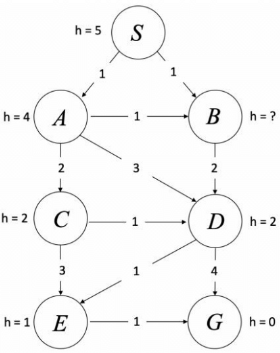
\includegraphics[width=0.3\linewidth]{fig/Astar.png}
\end{figure}

\begin{parts}
\part[3] With the heuristic values fixed for all nodes other than $B$, for which values of $h(B)$ will A* graph search be guaranteed to return the optimal path? (All heuristics are consistent.) Either fill in the lower and upper bound in the blank spaces below or write ``impossible” in two spaces.
$$\_\_\_\_ 4 \_\_\_\leq h(B)\leq \_\_\_ 4 \_\_\_\_$$

\part[3] Given the above heuristics, and choose (one of) the heuristic you answered in (a), write down the heuristic $h(B)$ you used. What is the order of the nodes that are going to be expanded in, assuming we run A* graph search on it.\\

$h(B)=\_\_\_ 4 \_\_\_$\\
Expand order:
%\vspace{1in}
\\$S,A,B,C,D,E,G$\\

\part[4] Based on (b), what path is returned?
\\$S,B,D,E,G$\\

\end{parts}
